\documentclass{article}
\usepackage[utf8]{inputenc}
\usepackage[T2A]{fontenc}
\usepackage[russian,english]{babel}
\usepackage{ragged2e}
\usepackage{graphicx} % Required for inserting images

\newtheorem{theorem}{Теорема}

\newtheorem{definition}{Определение}[section]

\graphicspath{{.}}

\title{Задание по курсу "ВвЧМ 24/25": Приближение функций}
\author{Павел Васильев, 213 группа}
\date{Декабрь 2024}

\begin{document}

\maketitle

\section{Постановка задачи}
Интерполяция - это способ нахождения промежуточных значений величины по имеющемуся дискретному набору известных значений.

Интерполяция использует значения некоторой функции, заданные в ряде точек, чтобы предсказать значения функции между ними. Перечисленные ниже методы предназначены для создания ряда с более высокой частотой наблюдений на основе ряда с низкой частотой. Например, вычислить ряд с квартальной динамикой на основе ряда годовых данных.

Многие задачи машинного обучения можно сформулировать через интерполяцию "неизвестной" функции
[1, 2]

Различные методы численного приближения и их теоретические обоснования можно найти в [3]

\subsection{Условия задачи}
Построить полином Лагранжа для следующих функций \(f_i(x)\) на отрезке \(x \in [-2,0]\):
\begin{enumerate}
    \item \(f_1(x) = T_5(x)\), где \(T_n(x) = 2xT_{n-1}(x) - T_{n-2}(x)\), \(T_1(x) = x\), \(T_0(x) = 1\)
    \item \(f_2(x)=|cos(5x)|e^{-x/2}\)
\end{enumerate}
В качестве узлов интерполяции выбрать узлы равномерной на [-2,0] сетки для количества узлов \(n=3,5,9,17\). Исследовать сходимость интерполяции. Найти максимальное отклонение \(\max|P_n(x)-f_i(x)|\) на равномерной сетке из 1001 узла. Построить графики исходных функций и их интерполянтов.

Подобрать более эффективный метод приближения функции для второй задачи.


\section{Используемые численные методы}
В решении были использованы методы приближения многочленами Лагранжа и кубическими сплайнами.

\begin{description}
    \item[Приближение многочленами Лагранжа.]

    В [3] представлено теоретическое обоснование данного метода, в частности, доказана теорема о приближении (n+1)-раз дифференцируемой функции.

    \begin{theorem}
        Пусть \(f \in C^{(n+1)}[a,b]\). Тогда
        \begin{equation}
            f(x) - L_n(x) = \frac{f^{(n+1)}(\xi(x))}{(n+1)!} \, \omega(x), \quad \omega(x) = \prod_{k=0}^{n} (x - x_k),
            \label{eq:lagrange_error}
        \end{equation}

        где
        \begin{equation}
            \min\{x, x_0, \ldots, x_n\} < \xi(x) < \max\{x, x_0, \ldots, x_n\}.
            \label{eq:placeholder}
        \end{equation}
    \end{theorem}

    Как будет видно, требование дифференцируемости здесь существенно, потому что иначе функция может и вовсе не приближаться полиномом.

    \item[Приближение кубическими сплайнами.]

    В [3] также представлен метод приближение сплайнами. Сплайн представляет собой кусочно заданный полином.
    \begin{definition}[Естественный сплайн]
        Кубический сплайн, обладающий следующим свойством
        \begin{equation}
            S''(x_0) = S''(x_n) = 0,
            \label{eq:placeholder_label}
        \end{equation}
        называется естественным сплайном.
    \end{definition}    

    \begin{theorem}
        Естественный сплайн существует и единственен.
    \end{theorem}

    Обозначим
    \begin{equation}
        h_k = x_k - x_{k-1}
    \end{equation}

    \begin{theorem}
        Пусть \(1 \leq j \leq 4\) и \(f \in C^j[a, b]\). Тогда
        \begin{equation}
            \|f - S_n\|_{C[a, b]} = O(h^j), \quad h \equiv \max_k h_k.
            \label{eq:example}
        \end{equation}
    \end{theorem}

    Таким образом, мы можем приближать функцию сплайнами, тогда нам становится проще бороться с негладкими функциями, если мы выберем точки разбиения там, где производная не существует.
\end{description}

\section{Результаты}

\subsection{Приближение многочленами Лагранжа}
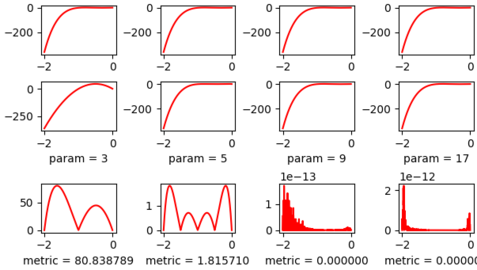
\includegraphics{Figure_102.png}

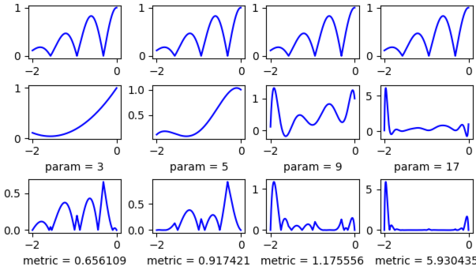
\includegraphics{Figure_103.png}

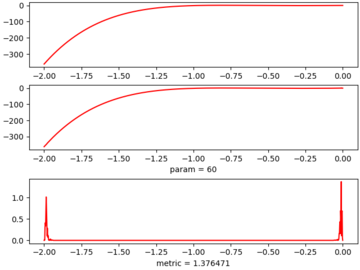
\includegraphics{Figure_104.png}

\subsection{Приближение сплайнами}
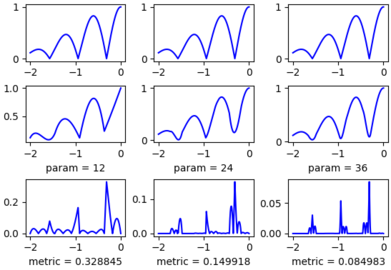
\includegraphics{Figure_101.png}

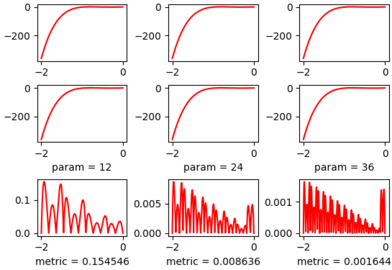
\includegraphics{Figure_100.png}

\subsection{Почему так?}
Как видим, первый способ позволяет довольно просто интерполировать многочлен, но ломается, когда мы пытаемся приблизить вторую функцию, но можно обратить внимание, что проблема возникает на границах (вблизи \(x = -2\) и \(x = 0\)), в остальном же функция приближается.

Метод приближения сплайнами позволяет обойти первый метод, когда уже при сетке из 12 точек, мы в разы улучшаем метрику.

Можно ещё заметить на рис.3, что при увеличении числа точек сетки, у нас возникают проблемы на границе, даже у полиномиальной функции, скорее всего из-за потери точности при множественных умножениях/делениях при нахождении коэффицентов полинома.

\subsection{Программная реализация}
Данные численные методы реализованы на языке Python с использованием NumPy, matplotlib.

Код хранится в репозитории: 
https://github.com/GoodDay-lab/practicum-numerical-method

\section{Выводы}
Таким образом, в ходе выполнения задания был реализован метод приближения полиномами Лагранжа и сплайнами. Было отмечено и теоретически доказано, что полиномы Лагранжа могут эффективно приближать функции \(f \in C^n[a,b]\), давая достаточно хорошую оценку. При этом совершенно неопределено поведение для негладких функций, и как мы видим, их они могут и вовсе не приближать. В таком случае можно использовать приближение сплайнами - кусочно-полиномиальными функциями. В этом случае оценка становится в разы лучше для негладких функций.


\section{Библиография}
\begin{enumerate}
    \item Хайкин С. "Нейронные сети. Полный курс", стр.82
    \item (url: https://education.yandex.ru/handbook/ml/article/mashinnoye-obucheniye)
    \item Тыртышников Е.Е. "Методы численного анализа", гл.12,13,14
\end{enumerate}

\end{document}


